\chapter{Designing the System}
	In the following chapter, the overall design of the system is discussed. First and foremost, the basic architechture is decided, based on the requirements. Then more detailed subjects are covered, such as how authentication will work, how the solution keeps the users' data safe, and generally how it will work under the hood - so to speak.

	\section{Architecture}
		As per the requirements specified in section \ref{sec:requirements} on page \pageref{sec:requirements} the solution will have to be distributed. As such, there are two primary basic paradigms which can be used: Peer-to-Peer and Client-Server. In the following sections the pros and cons of the two will be discussed, and a conclusion of which is more beneficial for the project will be made.

		\begin{figure}
			\centering
			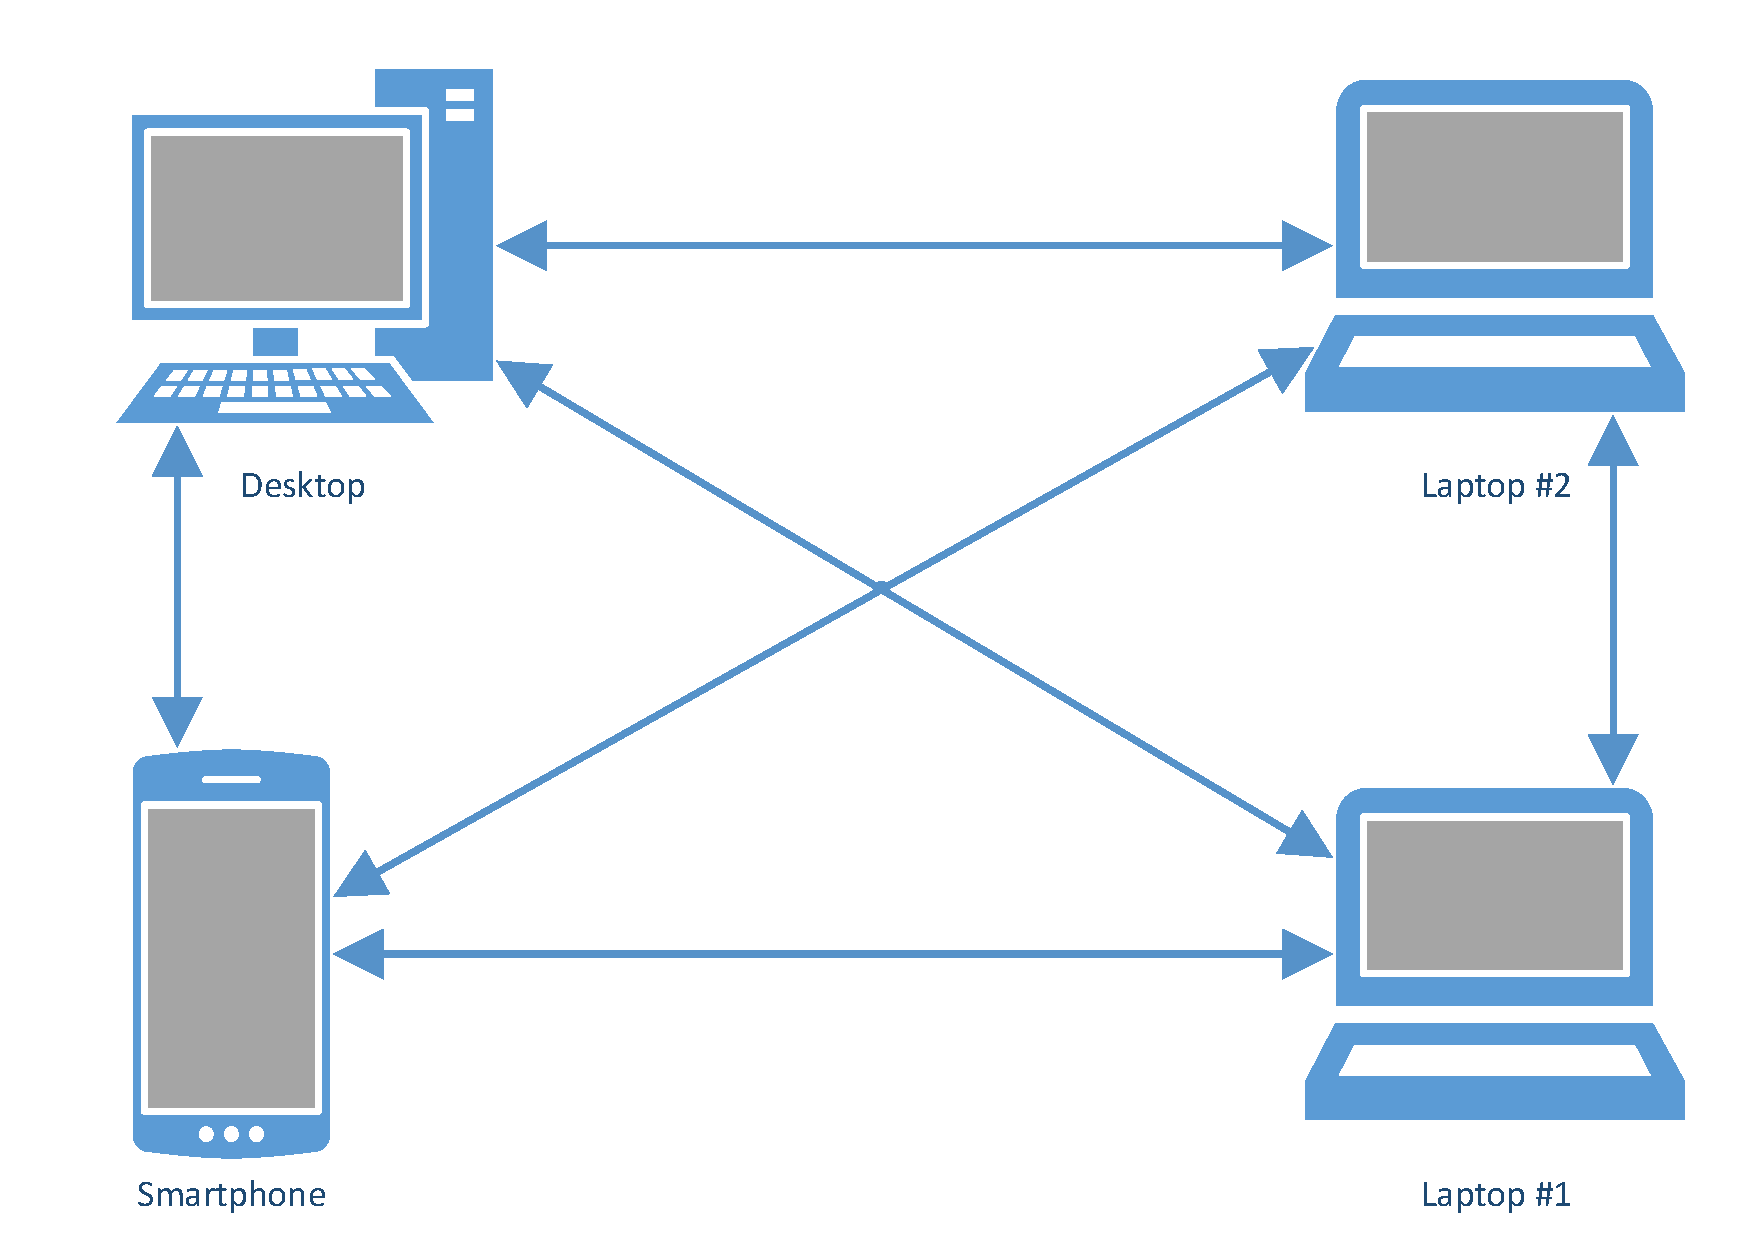
\includegraphics[width=\textwidth]{figures/design/PeerToPeer.pdf}
			\caption{Peer-to-Peer structure visualised.}
			\label{fig:peertopeer}
		\end{figure}

		\begin{figure}
			\centering
			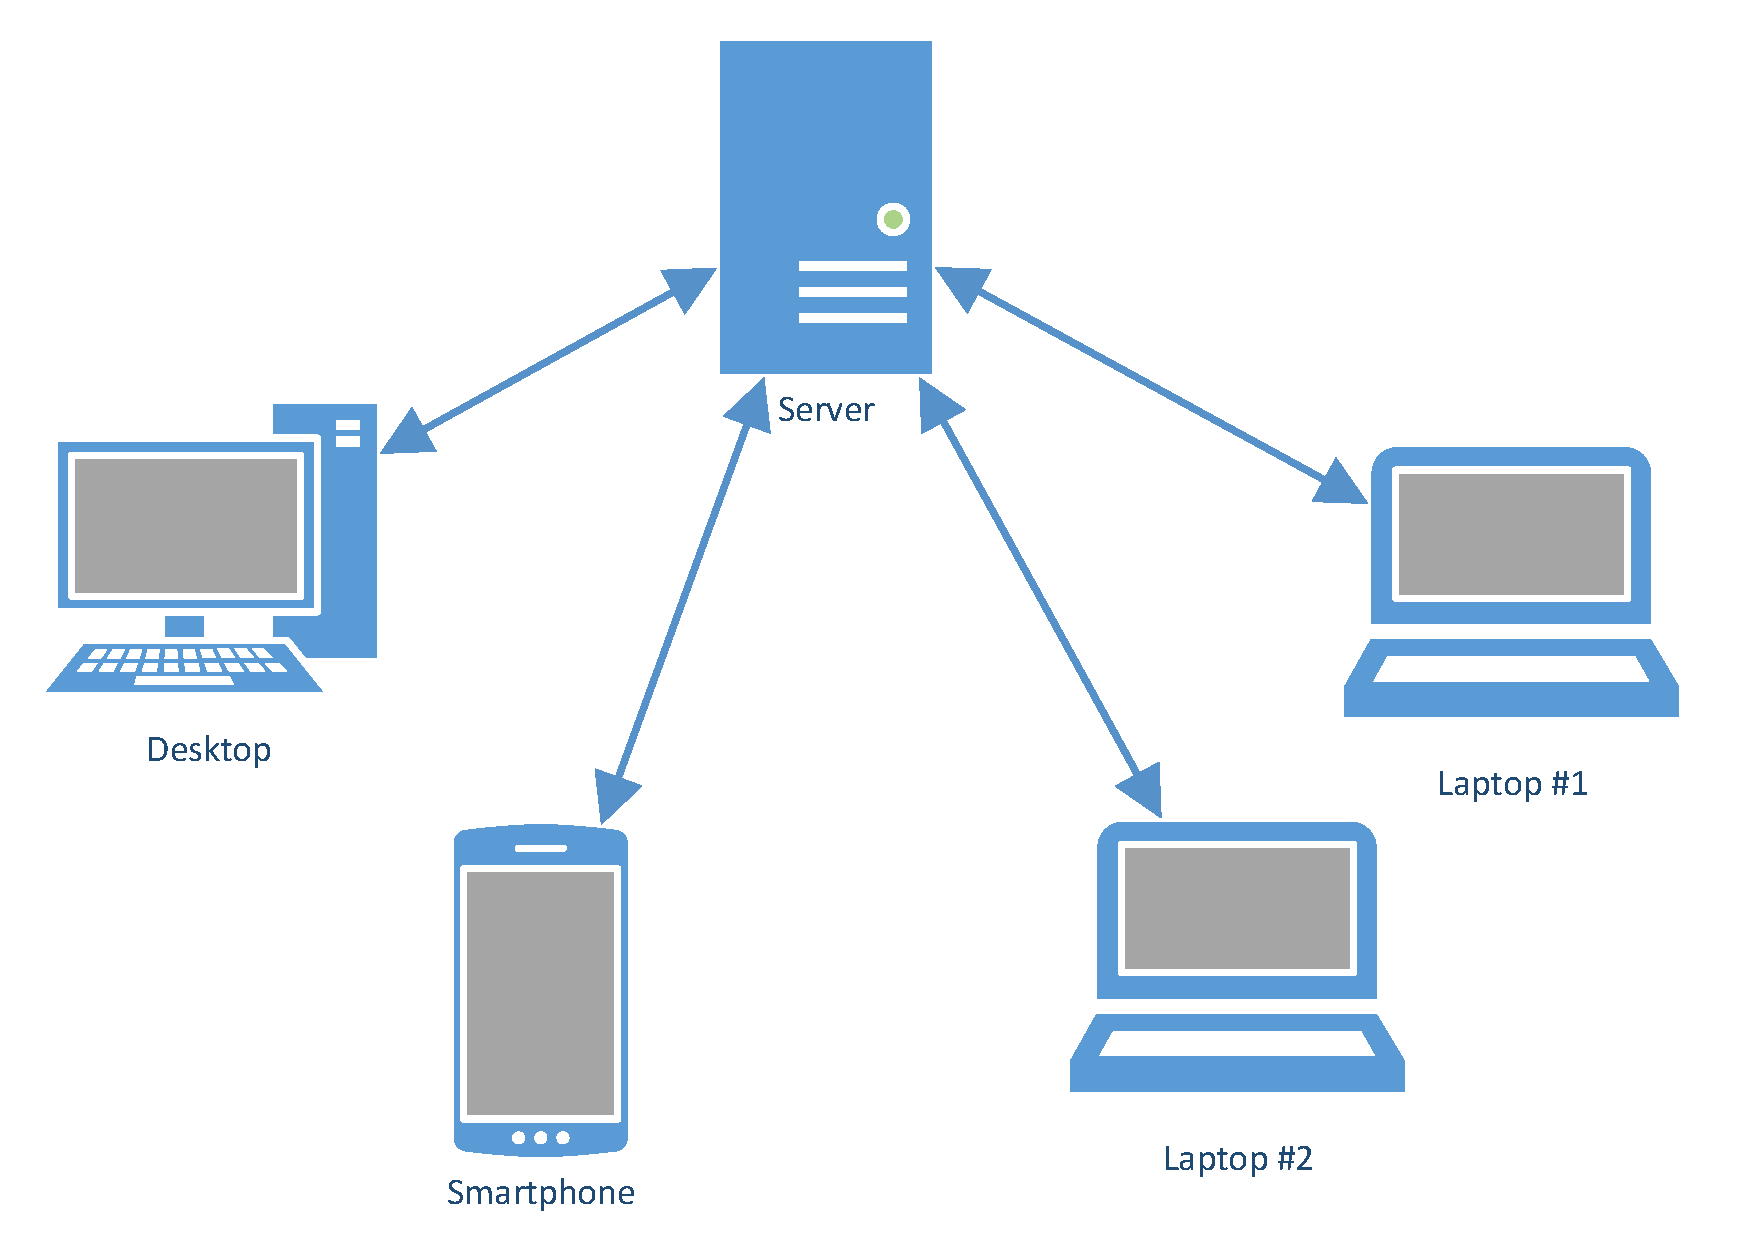
\includegraphics[width=\textwidth]{figures/design/ClientServer.pdf}
			\caption{Client-Server structure visualised.}
			\label{fig:clientserver}
		\end{figure}


		\subsection{Peer-to-Peer}
			Over the past few years, peer-to-peer technology has become ever so more appealing to the masses. Applications such as BittorrentSync applies peer-to-peer technology in an effort to synchronise data between devices. Such an approach could easily be adapted to the problem at hand. A number of a user's devices are online, and synchronises a local password database file between themselves, as visualised on figure \ref{fig:peertopeer} on page \pageref{fig:peertopeer}. This file is then accessed through a native application, on the target device. 

			This approach \emph{definitely} has the lowest overhead of the two: After all it is only devices that needs to have access to the passwords, that need to be setup, maintained, and running for it to be used. However, it does have some drawbacks. Most noticeable, that a native application is required for it to work. This means that for \emph{all} platforms an application needs to be developed. This, in returns, results in a much larger codebase, higher risk of bugs, and a risk of lower consistency across devices. Furthermore, the requirements of logging, as per section \ref{sec:requirements} on page \pageref{sec:requirements}, becomes a lot more difficult, if not to say impossible.

			Additionally, there is a pitfall using this approach. The synchronization requires at least \emph{one} peer with the newest version, to be online for it to work. Let us imagine a user, Paul. Paul has three devices he wish to synchronize passwords to: A desktop, a laptop, and a smartphone -- a very common scenario! Before leaving for a holiday, Paul updates a password on his desktop, while his laptop is closed. Since the smartphone is online at the time, the password is stored there and Paul is perfectly able to access it on his way to the airport. Since it's a long trip, Paul's smartphone runs out of battery along the way. ``No problem!'', Paul thinks and pulls out his laptop -- but oh no! Since the laptop has been offline ever since he left home, it has not received the updated password. And since it is the only online peer -- the desktop at home is turned off and the smartphone has run out of battery -- he can't fetch the newest version. 

			The scenario presented before, can be somewhat mitigated by creating an ``always on peer''. It is a peer in the network, which is always connected and thus always has the newest version available for other peers. However, doing this very much negates one of the strongest arguments \emph{for} this approach: The lower overhead.

		\subsection{Client-Server}
			The client-server paradigm has been the basic model used, since the dawn of the modern internet. When browsing facebook, accessing gmail, or posting a tweet, this is the paradigm employed. It is also the most widespread model used, by the solutions examined in chapter \ref{chap:analysis}.

			Using this approach, there would have to be a dedicated server, acting as the ``master storage'' of passwords. Each client then connects to this server and fetches the passwords. This type of connection is visualised on figure \ref{fig:clientserver} on page \pageref{fig:clientserver}. This does, however, come with its own drawbacks. Since all passwords are stored on a single server, it introduces the risk of a single point of failure. Should the server be compromised or is otherwise unavailable, passwords can not be retrieved \emph{(unless a local cache is used, but this is delving into implementation details)}. It also comes with overhead in form of cost and maintenance. A server will have to be maintained and run 24/7. However, as mentioned in section \ref{sec:privatecloud_cost} on page \pageref{sec:privatecloud_cost}, this can be achieved using low-power devices such as a Raspberry Pi, reducing the financial cost significantly.

			Finally, using the client-server paradigm counters the scenario presented in the previous section. When Paul updates the password from home, the updated password is stored on the server. When he uses his laptop, after his phone has died, it will fetch the updated password from the server.


		\subsection{Conclusion}
			After having weighed the pros and cons of the two approaches, it is decided that a classic client-server architecture will be used. It is deemed that it will create a more seamless experience for the user, and over all will be a more robust solution.

			Another argument why the client-server paradigm is preferable is that if the peer-to-peer paradigm is used, a native application is \emph{required}. This is not the case for the client-server paradigm. A web UI could serve as a front-end, creating a completely identical user experience across devices. But a native application could also be the solution, for the client-server application. Hence, this paradigm allows more freedom of implementation, than peer-to-peer does.

			From here on out, the solution will be split into two parts: The front-end \emph{(client)} and back-end \emph{(server)} -- two very common denominators.


	\section{Communicating}
		Having determined that the solution will be using the client-server paradigm, the next task is to determine how front-end and the back-end will communicate. There are a number of different available technologies and protocols readily available for use in such a scenario.

		One important fact, that needs to be stated that the back-end is practically equivalent to a web service. As such, 

		\begin{itemize}
			\item Representational State Transfer
			\item SOAP	
			\item Sockets
			\item Remote Procedure Calls
		\end{itemize}

		\subsection{Remote Procedure Call}
			Remote Procedure Calls, or RPC for short, was introduced by Birrell and Nelson \cite{birell1984} in 1984. The basic concept is to hide the implementation details of invoking a method remotely, for the user.

			The core concept of RPC is that invoking remote methods, are no different than invoking a local method. When the program invokes this method, the underlying software then makes the remote call, hiding these details from the programmer. This is the supposed strength of RPC: It is exactly like invoking a local method.

			An example of an RPC method, could be a method to get a user's data:
			\begin{verbatim}
				getUser(<ID>)
			\end{verbatim}

			For simplicity purposes, Remote Method Invocation is considered equivalent to RPC. Likewise implementations of RPC such as XML-RPC, Corba, and so forth, are considered under the same umbrella.

		\subsection{Representational State Transfer}
			Representational State Transfer, or REST for short, was introduced by Fielding and Taylor \cite{Fielding:2000:PDM:337180.337228} in 2000. REST is an architecture style for designing networked application. It is a stateless, client-server communication \emph{style}, which in most cases uses the Hypertext Transfer Protocol \emph{(HTTP)} protocol and the accompanying HTTP ``verbs''. Traditionally REST uses JSON as body encoding, however it is also possible to use XML.

			The core notion of REST is that resources are bundled in collections, on which the HTTP verbs are used. The API then exposes these collections as Uniform Resource Identifiers \emph{(URIs)} in what is commonly known as endpoints. Using the various HTTP verbs on these endpoints results in actions being invoked on said collections.

			These verbs are for example -- but not limited to-- \verb=GET=, \verb=POST=, \verb=PUT=, \verb=PATCH=, and \verb=DELETE=. These five verbs roughly translates to the basic CRUD operations, as listed on table \ref{tbl:verbs} on page \pageref{tbl:verbs}. So, for instance if one where to \verb=GET= the endpoint of \verb=/api/users= one would get the list of all users on the system. However, most of the time the distinction between \verb=PUT= and \verb=PATCH= is ignored, and \verb=PUT= is allowed to perform partial updates. Table \ref{tbl:rest_example} on page \pageref{tbl:rest_example} shows an example of an API on the \verb=users= resource, showing the result of the respective verbs and their payload. In the example the host of the endpoints have been removed, the prefix could for example be \verb=https://someapi.com/api=, so that an endpoint would be \verb=https://someapi.com/api/users=.

			\begin{table}
				\begin{tabular}{r|l}
					\verb=GET= 		& Read 				\\
					\verb=POST= 	& Create 			\\
					\verb=PUT= 		& Complete update 	\\
					\verb=PATCH= 	& Partial update 	\\
					\verb=DELETE= 	& Delete 			\\
				\end{tabular}

				\caption{How HTTP verbs maps to CRUD operations.}
				\label{tbl:verbs}

			\end{table}

			\begin{table}
				\begin{tabular}{p{0.15\textwidth} | p{0.30\textwidth} | p{0.15\textwidth} | p{0.25\textwidth}}
					Method & Request Body & Endpoint & Ouput \\
					\hline
					\verb=GET= & Empty & /api/users & List of all users \\
					\hline
					\verb=GET= & Empty & /api/users/1 & Details of user with ID of 1 \\
					\hline
					\verb=POST= & \{username:"Daniel", phone:"+45 88888888"\} & /api/users & Creates a new User with the name Daniel and the phone number +45 88888888 \\
					\hline
					\verb=PUT= & \{username:"John"\} & /api/users/1 & Updates the username of the user with ID of 1\\
					\hline
					\verb=DELETE= & Empty & /api/users/1 & Deletes the user with ID of 1\\
				\end{tabular}

				\caption{Example of HTTP verbs used on a REST API for the collection of users.}
				\label{tbl:rest_example}

			\end{table}

		\subsection{Simple Object Access Protocol}
			Simple Object Access Protocol \emph{(SOAP)} was developed by Goshein, Atkinson, Winer, and Box for Microsoft in 1997 \cite{soap_origin}. SOAP is considered an extension of XML-RPC and -- like its predecessor -- uses XML encoding. As implied by its successor SOAP is \emph{strictly speaking} considered an RPC, however due to its uniqueness from ``traditional'' RPCs it is considered separately.

			SOAP can be used with any number of protocols, due to its neutrality, however it is usually used with HTTP or SMPT. Web services relying on SOAP, usually publish a public definition of the available methods, using the Web Service Definition Language \emph{(WSDL)}. This can then be consumed by other clients, making integration with third parties much easier.

			Since SOAP used XML encoding, it is \emph{quite} verbose, and the pure data overhead is significant. Using the same example as from REST, getting the information for a user with ID 1 requires a rather large request body. the XML uses multiple namespaces, the \verb=xmlns= tags are required to define each of them, as \verb=SOAP= and \verb=m= respectively.

			\begin{verbatim}
				<SOAP:Envelope xmlns:SOAP="http://schemas.xmlsoap.org/soap/envelope/">
				    <SOAP:Body>
				        <m:getUser xmlns:m="https://someapi.com/api">
				            <userId>41</userId>
				        </m:getUser>
				    </SOAP:Body>
				</SOAP:Envelope>
			\end{verbatim}


		\subsection{Sockets}
			Underlying all of the previously described technologies are sockets. Sockets are the basic method computers communicate with eachother. Hence, of course it can be used for this purpose. However, there is a \emph{reason} the previous technologies exist: They take care of some of the heavy lifting. Defining a standard for communication, redundancy, standard errors, etc. are but some of the advantages of using either of the previously described technologies. As such, using sockets directly is dismissed without further arguments. 


		\subsection{Making A Choice}
			Making the final choice of how the solution will communicate is important. It sets limitation on future work, and could possibly influence design choices not yet even thought of. 

			First and foremost let us examine RPC. While it \emph{was} the go-to method for achieving the sort of communication which is needed in this project, the issue of implementation remains. Each platform will need its own unique implementation of whichever RPC standard that is chosen. And there is no guarantee that all of these will adhere to the specifications. Additionally, since its usage has become less widespread, it will also hinder further development and integration from third parties, down the line. As such, RPC is dismissed as a possible solution.

			This leaves SOAP and REST. SOAP is a very ``heavy'' tool, often used in commercial applications, due to its stricter nature. Because of the XML syntax, their payload is \emph{significantly} larger than that of REST using JSON. This results in SOAP being magnitudes slower than REST, cf. \cite{soap_vs_rest}. Additionally there is the matter of support and general adaptation. In the open-source community REST seems to have won the hearts of the crowd. More libraries and tools exists, for aiding in quick development of a RESTful API. This will also make for the optimal base, should other users choose to integrate the solution with their own projects.

			Hence, it is decided that a RESTful approach will be used.


	\section{Authentication}
		\subsection{OAuth1/2}
		\subsection{Basic Authentication}
		\subsection{Tokens}
			\subsubsection{Simple Web Tokens (SWT)}
			\subsubsection{JSON Web Tokens (JWT)}
		
		\subsection{Two-Factor Authentication}

	\section{Securing the API}

	\section{Encryption \& Data Security}
		\subsection{Pseudo Zero Knowledge}


	\section{Storing the Data}
		\section{SQL vs NoSQL}
		\section{SQLite}
	\section{Storage Scheme}

	\section{Naming the Solution}

